% Network perspective

To properly understand absorptive capacity we have to combine the resource-based view and the relational view of the firm because the absorptive capacity of a firm is partly determined by its ability to establish and maintain productive inter-organisational ties \citep{vanhaverbeke2007connecting}. Networks provide firms with access to knowledge, resources, markets, or technologies \citep{inkpen2005social}. Open innovation assumes critical knowledge resources span firm boundaries and are likely to be embedded in inter-firm routines and processes \citep{dyer1998relational,chesbrough2003open}. Investigating the antecedents and configuration of knowledge networks requires a methodology capable of dealing with relational data \citep{lusher2014cooperative}.  

\section{social networks}

Networks provide a way of thinking about social systems, one that focuses on the relationships among entities that make up the system \citep{borgatti2013analyzing,robins2015doing}. One can represent networks mathematically as graphs i.e. mathematical objects comprising a set of vertices and a set of edges that connect vertices \citep{newman2010networks}. Vertices represent actors or nodes in a social network. Actors can be individuals, groups, organisations, regions, nations, or even a group of countries. These may be distinguished by binary, categorical or continuous attributes. For example, consider an individual actor classified as female (binary attribute), who works for a particular organisation (categorical attribute), with a specific number of years work experience (continuous attribute). Edges represent relations or social ties between actors. Ties can be measured as directed or undirected and as binary or valued. Deciding whether to measure a tie as directed or undirected depends on the theoretical nature of the tie. For example, co-membership is inherently undirected whereas authority is essentially directed. Directed and undirected ties can be measured as binary ties that either exist or do not exist, or as valued ties that can be stronger or weaker, transmit more or fewer resources, or have more or less frequent contact \citep{scott2011sage}.\medskip

Different types of relations may exist between actors. Each type of relation gives rise to a corresponding network \citep{borgatti2013analyzing}. Measuring knowledge sharing ties would, for example, generate a knowledge sharing network. By assigning an attribute to the knowledge sharing tie, we can qualify the relationship in terms of the content or frequency of knowledge sharing. \medskip

Ties can be classified according to similarities between actors and by relational roles, cognition, and events \citep{borgatti2013analyzing}. Ties between actors who share something in common (e.g. spatial location, affiliated to the same body, participate in the same event, or share a common attribute) are referred to as similarity ties. Relational roles include kinship and other ties such as friendship, advice, and managerial ties. Relational cognition refers to ties that are affective (e.g. like or dislike another actor) or perceptual (e.g. belief about the other actor) in nature. Relational events refer to ties defined by specific social interactions (e.g. a transaction of some kind) and flows (e.g. knowledge flows).\medskip

Some ties are dependent on others. An example is friendship, which usually develops because of an pre-existing similarity tie (e.g. both actors live in the same neighbourhood, attend the same school, or work at the same place) or via a relational event tie (e.g. actors were introduced to each other at a specific event or worked together on a particular project). Another example is knowledge sharing. Actors are more likely to share  knowledge (relational event) with others who have common interests (similarity tie) or with other they trust (relational cognition).  


All enacted relationships or networks are embedded within formal arrangements \citep{kadushin2012understanding}.

 Informal interpersonal networks are thought to play a critical role in the knowledge transfer process \citep{reagans2003network}. More than two-thirds of all technical collaboration is done through informal interpersonal networks \citep{selnes2003promoting}. 



The interdependence of ties is what makes social systems complex and difficult to study.\medskip   
 

\section{Social network analysis}


Social network analysis uses various techniques to examine relations between social entities and the implications of these relationships \citep{wasserman1994social}. The aim of social network analysis is to examine patterns of relations, not just ties between pairs. To fully understand the implications of dyadic relations, one has to consider how these are shaped by broader patterns of social interaction \citep{scott2011sage}. This requires more than knowing how to measure basic characteristics of networks. A set of assumptions is needed to best describe and explain social phenomena of interest. One may apply an existing sociological theory to test hypotheses about social relations. Alternatively, one may use networks to explain specific outcomes or assess how social processes are influenced by network effects \citep{scott2011sage,borgatti2013analyzing}.\medskip
 
Positions and roles are key concepts in social network analysis.


%\subsubsection{Network notation}
%% from snijders 2011
%
%A social network is a structure of ties or relational variables between social actors. We shall consider mainly a fixed set {1,...,n} of actors, and variables Xij representing how actor i is tied to actor j. In some cases these will be directed in nature, so that Xij and Xji are different variables which may assume the same or different values. In other cases they will be non-directional in nature, so that Xij is necessarily equal to Xji. The most frequently employed and most strongly developed data structure is for binary variables Xij, where the value 1 (or 0) represents that there is (or there is not) a tie from i to j. Then the mathematical object constituted by the set {1,...,n} and the variables Xij is called a graph in the non-directed, and a digraph in the directed case. Actors are called the nodes and the ties are usually referred to as arcs or edges, depending on whether the graph is directed or not. It is usual to exclude the possibility of self-ties, so that the variables Xii are considered to be structural zeros.
%
%\subsubsection{Network dependencies}
%
%Reciprocation of directed ties is a basic feature of social networks. This will be reflected by dependencies between Xijand Xji. Theoretical accounts have been made for it from the points of view of social exchange theory (Emerson, 1972) and game theory (Axelrod, 1984). Reciprocation need not be confined to pairs, but can circulate in larger groups \citep{molm2007}. This then can lead to depen- dence in longer cycles such as Xij,Xjh,Xhi.
%
%Homophily, the tendency of similar actors to relate to each other \citep{mcpherson2001birds}. Theoretical arguments can be based on opportunity, affinity, ease of communication, reduced transaction costs and break-off risks, and organizational foci composed of similar individuals. This leads to a higher probability of ties being formed between actors with similar values on relevant covariates \citep{snijders2011statistical}.
%
%Transitivity of ties is expressed by the saying ‘friends of my friends are my friends’, and was proposed as an essential element of networks by Rapoport (1953a,b). Davis (1970) found large-scale empirical support for transitivity in networks. Transitivity is rooted deeply in sociology, going back to authors such as Simmel (1950) and elaborated more recently by Coleman (1990).
%
%If there is a tendency toward transitivity, the existence of the two ties Xij= Xjh= 1 will lead to an increased probability of the tie Xih= 1, the closure of the triangle. Concatenation of such closure events then can lead also to the existence of larger connected groups. Transitivity therefore also has been called clustering (Watts, 1999).
%
%A natural measure for the transitivity in a graph is the number of transitive triangles, ?i,j,hxijxjhxih (to be divided by 6 in the case of nondirected graphs). A natural normalization is to divide by the number of potentially closed triads, as proposed by Frank (1980), ?i,j,hxijxjhxih?i,j,hxijxjh . (1) In directed graphs, transitivity can have two faces: it may point to a hierar- chical ordering or to a clustered structure. These two can be differentiated by the aid of the number of 3-cycles,?i,j,hxijxjhxhi. A relatively high number of 3-cycles points toward clustering, a relatively low number to- ward hierarchy. Davis (1970) found empirically that social networks tend to contain a relatively low number of 3-cycles, indicating the pervasiveness of hierarchies in social networks.
%
%
%
%Degree differentials, some actors being highly connected and others hav- ing few connections, was studied since the last 1940s for communication networks by Leavitt, Bavelas, and others, and this led to models for node centrality reviewed by Freeman (1979). An important theoretical account was the rich-get-richer phenomenon, or Matthew effect, elaborated in the context of bibliographic references by de Solla Price (1976). This will lead to a high dispersion of the nodal degrees, which then may further lead to core-periphery structures (Borgatti and Everett, 1999) or various other types of hierarchical structures.
%
%Hierarchies in directed networks, as exhibited by high transitivity and few 3-cycles, may be local or global. A global hierarchy will be indicated by the ordering of the in-degrees and/or out-degrees, where the typical pattern e.g., in esteem or advice asking, is directed from low to high. In a purely global hierarchy, which can be seen, e.g., in some advice networks, in a statistical model the degree differentials will be sufficient to explain the low number of 3-cycles. But local hierarchies are possible in directed networks even when the in-degrees and out-degrees exhibit rather little variability.
%
%\subsubsection{Exponential random graph models}
%
%
%The nature of networks leads to dependence between actors, and also to dependence between network ties \citep{snijders2011statistical}. Statistical modelling on the other hand is normally based on assumptions of independence. 
%
%The complicated nature of network dependencies has delayed the development of statistical models for network structures.
%
%Exponential random graph models are a class of statistical model for social networks originally developed by \citet{frank1986markov} and refined by \citet{wasserman1996logit} and \citet{pattison1999logit}. 
%
%The array X = (Xij) of random variables, which can also be regarded as a stochastic graph, is a Markov graph if for each set of four distinct nodes {i,j,h,k}, the random variables Xijand Xhk are conditionally independent, given all the other random variables in X. This seems a plausible kind of conditional independence, suitable for social networks. Frank and Strauss (1986) proved that this Markov dependence for a random nondirected graph, with the additional requirement that the probability distribu- tion is invariant under permutation of the nodes, is equivalent to the possibility to express the probability distribution of the graph by P{X = x} =exp?θL(x) +?n−1k=2σkSk(x) + τT(x)? κ(θ,σ,τ) (4) where L(x) =?i<jxij is the edge count, T =?i<j<hxijxjhxihis the triangle count, and Sk=?i?j1<j2<...<jkxij1xij2...xijkis the k-star count (with S1(x) = L(x)).
%
%The statistical parameters in this model are θ,σ2,...,σn−1, and τ. Finally, κ(θ,σ,τ) is a normalization constant to let the probabilities sum to 1. The fact that the logarithm of the probability is a linear combination of parameters and statistics makes this into an exponential family of distributions (Lehmann and Romano, 2005), an important class of statistical models for which many theoret- ical properties are known. The statistics are the so-called sufficient statistics, as they contain all information in the data about the values of the parameters. The sufficient statistics here are subgraph counts, the frequency in the graph of small
%
%configurations: here, edges, k-stars, and triangles. The number of k-stars can be expressed as Sk(x) = n?i=1?xi+k?, (5) which implies that the vector of k-star counts Sk(x) for k = 1,...,K are a linear combination of the first K moments 1 n n?i=1Xki+ (k = 1,...,K) of the degree distribution. Thus, if σk= 0 for all k larger than some value K, in a distribution of graphs according to (4) each graph with the same moments of order up to K of the degree distribution, and the same number of triangles, is equiprobable. Often this model is used while including only a few of the σk parameters for low k, so that the degree distribution is characterized by a few low-order moments such as the mean, variance, and skewness. Frank (1991) and Wasserman and Pattison (1996) generalized the Markov graph model by proposing that the exponent in (4) could contain in principle any statistic, thus allowing any kind of dependence between the tie variables: Pθ{X = x} =exp??kθksk(x)?κ(θ), (6) where the sk(x) can be any statistics depending on the network and observed covariates. They can be specified so as to reflect the research questions and to obtain a good fit between model and data. This model can represent in principle any distribution on the space of graphs that gives positive probability to each possible graph – although such a representation will not necessarily be parsimonious or tractable. This model was called the p∗model by Wasserman and Pattison (1996); more recently it has also been called the Exponential Random Graph Model (‘ERGM’). An important subclass is obtained when the sufficient statistics sk(X) are subgraph counts (such as is the case for the Markov model). Such models can be obtained from conditional independence assumptions (of which, again, Markovian dependence is one example) based on an application of the Hammersley-Clifford theorem, as proved in Wasserman and Pattison (1996). Examples are the neighbourhood models of Pattison and Robins (2002) and the models excluding ‘action at a distance’ discussed by Snijders (2010). An overview of the Exponential Random Graph Model is presented in Robins et al. (2007) and in the monograph Koskinen et al. (2011).
%
%Exponential Random Graph Models, when using subgraph counts as sufficient statistics, are based on conditional independence assumptions between the ob- served tie variables. There is a large flexibility in specifying the sufficient statis- tics, and this can give insights in dependence structures between the ties in the network. An example is the elaboration of this type of model for directed net- works by Robins et al. (2009), where many different dependence structures are possible because directions of ties can be combined in so many ways. One of the examples treated is a network of negative ties (difficulties in working with the other person), where the specific dependence structures may be of great interest.
%
%researchers who are interested in detailed dependence structures might profit more from applying Exponential Random Graph Models.
%
%Exponential Random Graph Models in the difficulty to achieve convergence of the algorithm. This may change as better computational methods become available. On the other hand, the complexity of dependencies in networks is so high that modeling large networks in a way that passes the high requirements of a good statistical fit seems intrinsically difficult to achieve.
%
%Exponential random graph models allow one to simultaneously estimate the effect of factors at the node, dyad and structural network levels \citep{broekel2013explaining}. They are useful for analysing the determinants of the structure of inter-organizational networks. Exponential random graph models serve as a pattern recognition device for predicting why social network ties occur. Network configurations are patterns of social network ties assumed to represent underlying social processes or mechanisms \citep{lusher2014cooperative}. Exponential random graph models provide a principled way of making inferences about the association of actor attributes and network ties because it can distinguish between whether ties were formed due to the attributes of the actors or whether simply the actor’s centrality is the result of being embedded within many purely structural network structures \citep{lusher2014cooperative}. Exponential random graph models permit differentiation between structural network effects and processes related to actor attributes. Purely structural effects reflect endogenous processes in which ties form due to the presence or absence of other ties. Ties may also form due to exogenous factors including actor attributes ...and are known as actor-relation effects. Table \ref{} provides a summary of purely structural and actor-relation effects that can be evaluated using exponential random graph models. 
%
%Exponential random graph models are particularly well-suited to this study, which is concerned about the individual, dyadic and organisational antecedents to knowledge sharing and knowledge creation in open innovation networks.
%
%\section{network centrality}
%
%A growing body of research demonstrates that possessing a central network position predicts knowledge sharing in positive ways (e.g., Ander- son, 2008; Burt, 1992; Freeman, 1979; Tsai, 2001). Every tie in an employee’s network represents a channel through which knowledge may flow to and from that employee (Anderson, 2008). Because of their more numerous network ties, employees in central network positions have more relationships to draw on for the purpose of knowledge sharing. As a consequence of their extensive knowledge- sharing activity, employees who possess central network positions are likely to accumulate work- related knowledge, which positively affects not only their performance, but also their future knowl- edge sharing with colleagues (Sparrowe et al., 2001). \citep{reinholt2011central}
%
%Hierarchy is an important dimension of social structure that indirectly influences social capital by shaping the structure of social relations \citep{adler2002social}.
%
%\section{Application}
%
%Examining the configuration of knowledge sharing ties should shed light on social mechanisms driving knowledge acquisition and knowledge assimilation (potential absorptive capacity). Likewise, the configuration of idea generation ties should provide insight on social mechanisms driving knowledge transformation and knowledge exploitation (realised absorptive capacity).
%

\section{Networked innovation}

Granovetter (1973) contends weak ties provide actors better access to new information and opportunities. Strong ties inhibit the flow of information from diverse distant sources. Sparse networks with an abundance of structural holes will allow strategically placed individuals to access diverse information and increase innovation output (Burt 2004). However, networks with fewer structural holes promote trust generation and reduce opportunism, leading to more productive collaboration from the perspective of resource sharing (Ahuja 2000). Burt (2001) believes brokerage across structural holes in the disconnected network is the source of value, but closure is critical to realising the value buried in structural holes. Strong ties are more effective than weak ties in enhancing knowledge transfer and learning as well as an individual’s ability to benefit from collaborating with diverse partners (Phelps et al. 2012; Rost 2011). Clarifying the implications of closed versus disconnected network structures for various organisational outcomes is important to our understanding of network resources (Ahuja 2000).
Individuals who are both strong knowledge producers and great collaborators enhance their firm’s innovative output (Grigoriou and Rothaermel 2013). Relational stars provide firm-level knowledge advantages not only through their own superior recombinant efforts, but also through their capacity to make others around them more effective at knowledge recombination. Relational stars possess strong combination of both human and social capital, that is, a strong individual-level productivity performance combined with a highly consequential network position (Grigoriou and Rothaermel 2013). 
Diversity of knowledge and perspectives provided by bridging ties does not automatically translate into the generation of innovations (Ahuja 2000). Quality of relationships, and how these are managed, affects the ability of an individual to network strategically and expose them to opportunities (Uzzi 1997). Tortoriello and Krackhardt (2010) investigate the paradox in which diversity of knowledge and information available across organisational boundaries is necessary to spur innovation, yet at the same time may be a barrier for successful knowledge sharing and integration. Advantages stemming from bridging ties are contingent upon the configuration or microstructure of the ties forming the bridge (Tortoriello and Krackhardt 2010; Tortoriello 2014). Common third-party ties facilitate shared understanding, reduce friction due to differences in understanding, and promote cooperation and coordinated actions that are necessary to integrate and take advantage of diverse sources of knowledge (Tortoriello and Krackhardt 2010). Such brokerage is a crucial means by which intra- and inter-organisational networks evolve, expand and drive change (Obstfeld et al. 2014). The relationship between external knowledge and an individual’s ability to generate innovations is contingent on the type of knowledge and the individual’s position in the internal knowledge-sharing network (Tortoriello 2014; Tortoriello 2006). 


\section{Brokerage}

\citet{gould1989structures} define a brokerage role as the position of j in an (i,j),(j,k) two-path with no (i,k) edge i.e. an intransitive triple. Adding a (k,i) edge to the representing cyclic closure does not undermine j's brokerage role. Brokerage involving transitive closure is not really brokerage in a cross-sectional context (Butts, personal communication).


\begin{table}[]
	\small
	\centering
	\caption{Gould-Fernandez brokerage roles}
	\label{gf_params}
	\begin{tabular}{@{}lcl@{}}
		\toprule
		\multicolumn{1}{c}{Role} & \multicolumn{1}{c}{Graphic} & \multicolumn{1}{c}{Explanation} \\ \midrule
		b\textsubscript{O} (liaison role)			&  \begin{minipage}{.2\textwidth} \centering 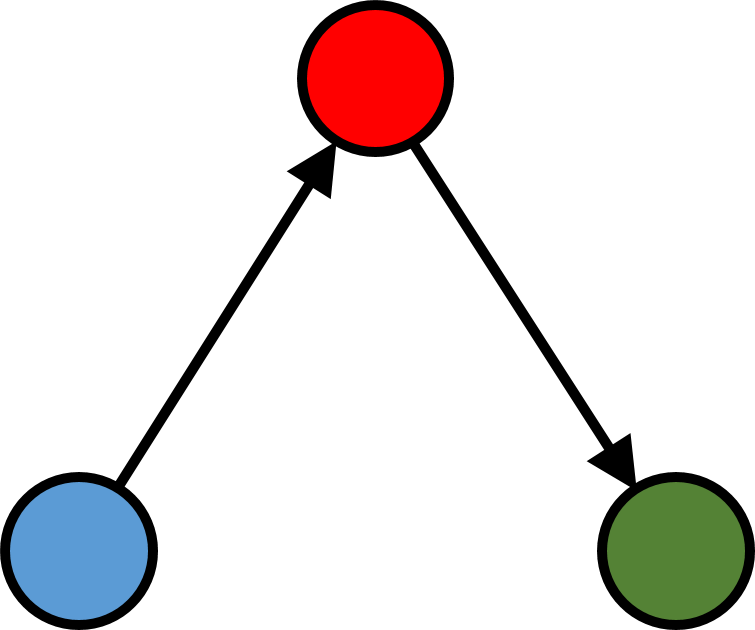
\includegraphics[width=0.4\linewidth]{Images/b_O} \end{minipage}	& \begin{tabular}[c]{l}Broker mediates contact between two\\ individuals from different groups,\\ neither of which is the group to\\ which he or she belongs.\end{tabular}\\ [10ex]
		b\textsubscript{IO} (representative role)	& \begin{minipage}{.2\textwidth} \centering 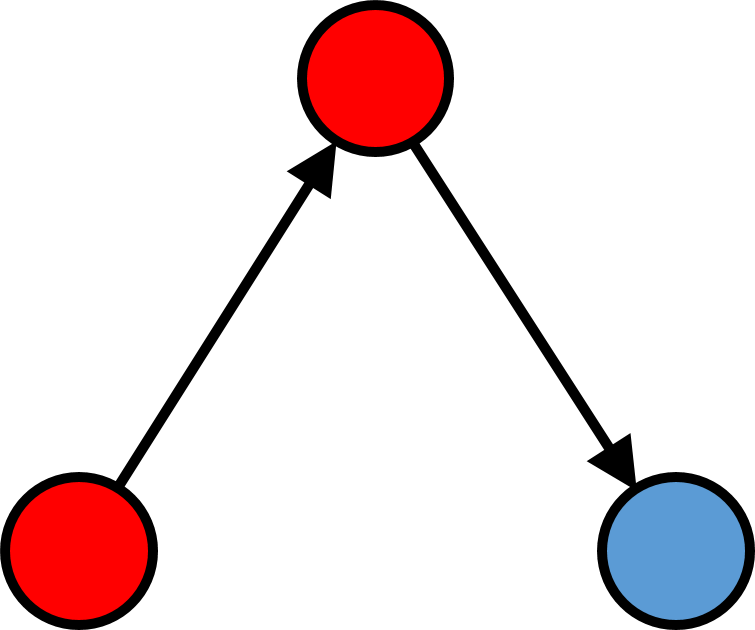
\includegraphics[width=0.4\linewidth]{Images/b_IO} \end{minipage}   & \begin{tabular}[c]{l}Broker mediates an outgoing contact\\ from an in-group member to an\\ out-group member.\end{tabular}\\ [10ex]
		b\textsubscript{OI} (gatekeeper role)		& \begin{minipage}{.2\textwidth} \centering 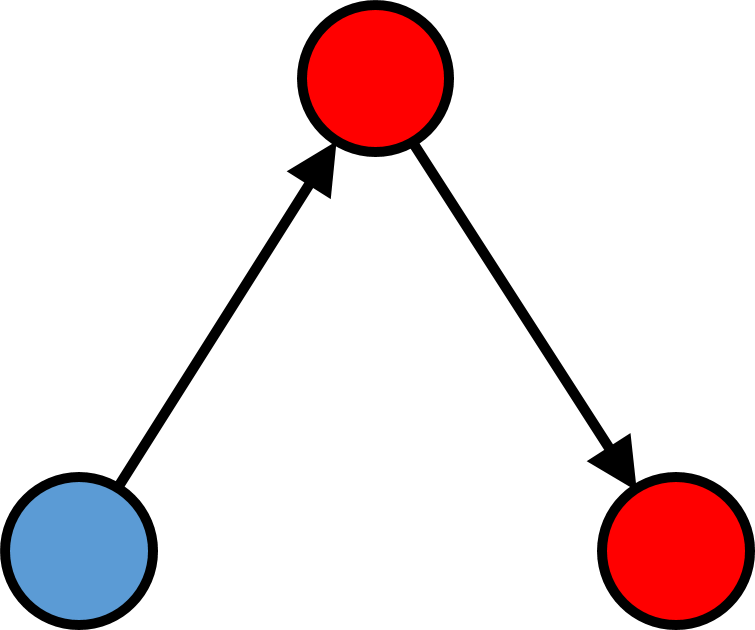
\includegraphics[width=0.4\linewidth]{Images/b_OI} \end{minipage}   & \begin{tabular}[c]{l}Broker mediates an incoming contact\\ from an out-group member to an\\ in-group member. \end{tabular}\\ [10ex]
		w\textsubscript{O} (itinerant broker)		&  \begin{minipage}{.2\textwidth} \centering 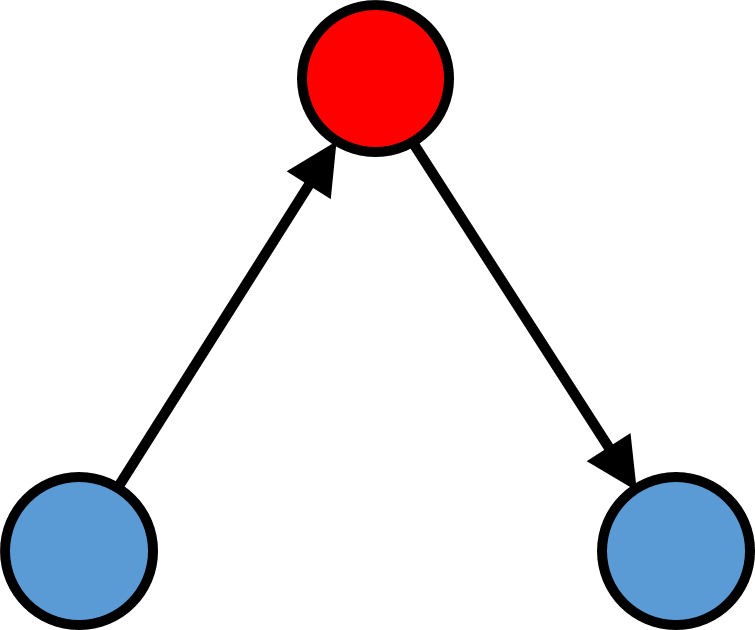
\includegraphics[width=0.4\linewidth]{Images/w_O} \end{minipage}   & \begin{tabular}[c]{l}Broker mediates contact between two\\ individuals from a single group to\\ which he or she does not belong. \end{tabular}\\ [10ex]
		w\textsubscript{I} (coordination role)		& \begin{minipage}{.2\textwidth} \centering 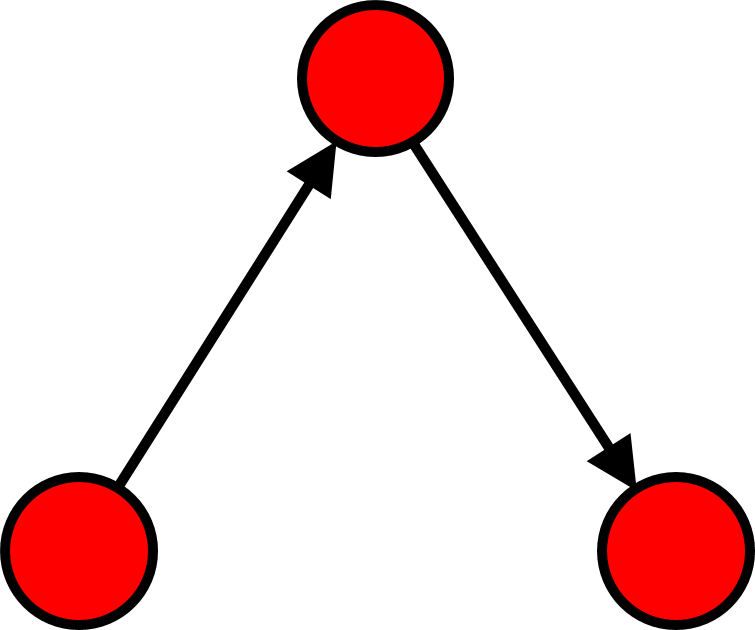
\includegraphics[width=0.4\linewidth]{Images/w_I} \end{minipage}    & \begin{tabular}[c]{l}Broker mediates contact between two\\ individuals from his or her own\\ group. \end{tabular}\\ 
		\bottomrule
	\end{tabular}
\end{table}

